%%
%% 研究報告用スイッチ
%% [techrep]
%%
%% 欧文表記無しのスイッチ(etitle,eabstractは任意)
%% [noauthor]
%%

%\documentclass[submit,techrep]{ipsj}
\documentclass[submit,techrep,noauthor]{ipsj}


% \usepackage[dvips]{graphicx}
\usepackage[dvipdfmx, hiresbb]{graphicx}
\usepackage{latexsym}
\usepackage{amsmath}
\usepackage{enumitem}
\usepackage{amssymb} 
\usepackage{url}

\newcommand{\todo}[1]{\colorbox{yellow}{{\bf TODO}:}{\color{red} {\textbf{[#1]}}}}
\newcommand{\ihara}[1]{\colorbox{green}{{\bf IHARA}:}{\color{blue} {\textbf{[#1]}}}}

\def\Underline{\setbox0\hbox\bgroup\let\\\endUnderline}
\def\endUnderline{\vphantom{y}\egroup\smash{\underline{\box0}}\\}
\def\|{\verb|}
%

%\setcounter{巻数}{59}%vol59=2018
%\setcounter{号数}{10}
%\setcounter{page}{1}


\begin{document}


\title{強化学習を用いたScratchにおける\\
リミックス元作品のCTスコア予測}

% \etitle{How to Prepare Your Paper for IPSJ SIG Technical Report \\ (version 2018/10/29)}

\affiliate{WU}{和歌山大学\\
Wakayama University, 930 Sakaedani, Wakayama 640--8510, Japan}



\author{堀尾 桃夏}{Horio Momoka}{WU}[momo5588.school@gmail.com]
\author{伊原 彰紀}{Ihara Akinori}{WU}[ihara@wakayama-u.ac.jp]

\begin{abstract}
本研究は,ビジュアルプログラミング言語Scratchにおいて,リミックス元作品のコンピュテーショナル・シンキング(CT)スコアを予測する手法を提案する.
他者の作品を複製・編集するリミックス機能が,学習者のCTスコア向上に有効であるが,その効果はユーザの学習経験によって異なることが従来研究で示されている.
本研究では,Scratchのユーザが作品制作した過程をマルコフ決定過程として捉え,強化学習を用いて
ユーザの学習経験に適した\todo{「選択する」の方がいい?}リミックスした元の作品のCTスコアを予測するモデルを構築する.実験の結果,\todo{XXを明らかにした}.
\end{abstract}


%
\begin{jkeyword}
    {Scratch,ビジュアルプログラミング,強化学習}
\end{jkeyword}
%

%\begin{eabstract}
%This document is a guide to prepare a draft for submitting to IPSJ
%Journal, and the final camera-ready manuscript of a paper to appear in
%IPSJ Journal, using {\LaTeX} and special style files.  Since this
%document itself is produced with the style files, it will help you to
%refer its source file which is distributed with the style files.
%\end{eabstract}
%
%\begin{ekeyword}
%IPSJ Journal, \LaTeX, style files, ``Dos and Dont's'' list
%\end{ekeyword}

\maketitle

%1
\section{はじめに}

日本では2020年度から小学校のプログラミング教育の必修化,2021年度から中学校の技術分野において,プログラミングに関する内容の充実,2022年度から高等学校の情報科において,共通必履修科目「情報1」の新設がされている\cite{monkashou}.しかし,指導者の情報不足や人材不足,予算不足などの指導者に対する問題が複数挙げられた\cite{monkashou2}.以前からプログラミング教育に力を注いでいるアメリカでは,Scratch\footnote{Scratch: \url{https://scratch.mit.edu/}}\cite{resnick2009scratch}と呼ばれるプログラミング初学者向けのビジュアルプログラミング言語を通してプログラミング教育を行っている.Scratchは「繰り返す」などの命令処理をもつブロックを,ジグソーパズルのように組み合せることで作品を完成させる.さらに,完成した作品はオンライン上に公開することができ,公開されている他ユーザの作品は,見る,使うだけでなく,複製し,編集することも可能である.この機能はリミックスと呼ばれる.

ビジュアルプログラミングは,プログラミング初学者が取り組みやすい環境を提供し,コンピュテーショナル・シンキング (CT) \cite{wing2006computational}スキルの向上を目的としている.学習や操作のハードルが低いため,プログラミングの入門学習として有効である.また,バグが少なく,直観的な操作のみでプログラミングをすることができるため,ユーザが短期間で作品を完成させやすく,達成感を得やすいという特徴をもつ.
% 近年では,情報化社会の進展に伴い,プログラマー不足が深刻な問題となっている.ビジュアルプログラミング言語の活用はその課題解決の第一歩になると考えられる.
しかし,プログラム作成を通して身につけたCTスキルを自身で評価・把握することは困難である.Morenoらは作品に使用されているブロックに基づき,CTスキルを計測するDr.Scratch\cite{moreno2015dr}を開発している.Dr.Scratchは,論理,制御フロー,同期,抽象化,データ表現,ユーザ対話性,並列処理の7つの概念に基づいて作品評価を行う.また,各概念を0点から3点の合計21点とし,CTスコアとして評価する.表\ref{CTscoreTable}に各概念の評価方法を示す.CTスコアを3つの区分に分類し,0点から7点をBasic,8点から14点をDeveloping,15点から21点をMasterとして評価する.
% 本論文ではDr.Scratchを用いて,CTスキルを定量的に評価する.

%--------------------------
\begin{table*}[t]
    \centering
    \caption{CTスコア概念\cite{hashitani2022scratch}}
    \label{CTscoreTable}
    \scalebox{0.8}{
    \begin{tabular}{c|c|c|c|c}
    \hline
    CTスキルの概念 & 0点 & 1点 & 2点 & 3点
    \\ \hline
    抽象化 & - &
    \begin{tabular}{c}
    2つ以上の\\スクリプトを使用
    \end{tabular}
    & 定義ブロックを使用 & クローンブロックを使用
    \\ \hline
    並列 & - & 
    \begin{tabular}{c}
    緑の旗ブロックを\\2個以上使用 
    \end{tabular}
    & 
    \begin{tabular}{c}
    オブジェクトへのクリックにより\\2つ以上のスクリプトを\\同時に実行する機能を実装
    \end{tabular}
    & 
    \begin{tabular}{c}
    イベント動作により\\2つ以上のスクリプトを\\同時に実行する機能を実装
    \end{tabular}
    \\ \hline
    論理 & - & Ifブロックを使用 & If elseブロックを使用 & 論理演算ブロックを使用
    \\ \hline
    同期 & - & 待機ブロックを使用 &
    \begin{tabular}{c}
    メッセージ受信により\\プログラムを停止する機能を実装
    \end{tabular}
    &
    \begin{tabular}{c}
    指定条件を満たすまで\\プログラムを停止する処理を実装
    \end{tabular}
    \\ \hline
    フロー制御 & - &
    \begin{tabular}{c}
    2個以上の処理ブロックを\\連結して使用
    \end{tabular}
    &
    \begin{tabular}{c}
    指定回数/回数無制限の\\繰り返しブロックを使用
    \end{tabular}
    &
    \begin{tabular}{c}
    指定条件までの\\繰り返しブロックを使用
    \end{tabular}
    \\ \hline
    ユーザ対話性 & - & 緑の旗ブロックを使用 &
    \begin{tabular}{c}
    ユーザの入力を伴う\\ブロックを使用
    \end{tabular}
    &
    \begin{tabular}{c}
    マイクやビデオなどの\\作用を伴うブロックを使用
    \end{tabular}
    \\ \hline
    データ表現 & - &
    \begin{tabular}{c}
    オブジェクトの\\プロパティを編集
    \end{tabular}
    & 変数ブロックを使用 & リスト変数ブロックを使用
    \\ \hline
    \end{tabular}
    }
\end{table*}
%--------------------------

従来研究では,Yangら\todo{引用}と橋谷ら\todo{引用}がリミックスについて分析している.これらの研究では,制作した作品数が同じユーザの中で,\todo{$\leftarrow$母数があってる?}リミックスによって作品を制作した経験を有するユーザは,経験のないユーザと比較して,使用するブロックの種類数およびCTスコアが高い傾向にあることを明らかにしている.しかし,リミックスの経験を有する全てのユーザのCTスキルが向上しているとは限らない.
% 本研究の事前分析において,特にCTスキルが低いユーザはブロックの種類数とCTスコアが増加することを明らかにした(\todo{X}章を参照).

% ず,極端に難易度が高い作品をリミックスしてもCTスキルへの効果が少なく,ユーザのCTスキルに適した難易度の作品のリミックスがCTスキル向上に寄与していると考える.\todo{$\leftarrow$これは妄想?}

本研究では,ユーザのCTスキルが向上する\todo{「選択する」か「向上する」かどっち?}リミックスした元の作品のCTスコアを予測するモデルを構築する.従来研究において,Fesakisらはリミックス元作品の協調性フィルタリングによるユーザ類似度でリミックス作品を推薦するという手法を提案している\todo{引用}.しかし当該手法では,類似したユーザがいない場合に推薦することができず,CTスキル向上に寄与しない作品を推薦することもある.現状のScratchは,キーワード検索のみで作品を検索するため,ユーザのCTスキルに適した作品を見つけることはできない.これらの課題を解決するため,ユーザが作品制作した過程をマルコフ決定過程として捉え,強化学習を用いてユーザが選択する\todo{ユーザのCTスキルが向上する?}リミックス元作品のCTスコアを予測するモデルを構築する.本研究では2つのReseach Question(RQ)に回答する.

\noindent\textbf{RQ1: }ユーザの熟練度によってリミックスの影響は異なるか?\\
\noindent\textbf{RQ2: }強化学習によるモデルは,リミックス元作品のCTスコアを適切に予測できるか?


以降,\ref{sec:related}章で従来研究について述べ,\ref{sec:dataset}章では本研究で使用するデータセットについて述べる.続く\ref{sec:preAnalysis}では,\ref{sec:rq1}章,\ref{sec:rq2}章では本研究のRQの目的と手法,結果,考察を述べ,最後に\ref{sec:conclusion}章で本論文をまとめる.

%%%%%%%%%%%%%%%%%%%%%%%%%%%
\section{従来研究}\label{sec:related}
%%%%%%%%%%%%%%%%%%%%%%%%%%%
従来研究では,Yangら\todo{引用}と橋谷ら\todo{引用}がリミックスがユーザのCTスキルにどのように影響するのかを調査した.リミックスをすることで使用するブロックの種類数が増加すること,また,CTスコアが向上することがわかった.しかし,必ずしもブロックの種類数が増加したりCTスコアが向上したりするとは限らない.加えて,リミックスによってCTスキルが向上したユーザの割合は示されておらず,どの熟練度のユーザに有効であるかは明確でない.

Fesakisらはリミックス元作品の協調性フィルタリングによるユーザ類似度でリミックス作品を推薦するという手法を提案した\todo{引用}.類似性を測定することができるJaccard係数を利用し,ユーザのリミックス元作品の一致不一致に重み付けを行い,多次元尺度構成法を用いることで類似関係を視覚化し,類似しているユーザを見つけ出した.例えばユーザAとユーザBが類似しているとすると,ユーザAがリミックスした作品かつ,ユーザBがリミックスしたことのない作品をユーザBに推薦する手法である.しかし,従来手法では類似したユーザがいない場合の推薦が不可能であることと,CTスキル向上に寄与しない作品まで推薦してしまう可能性が考えられる.

\todo{従来研究は増やしたい}

\todo{本研究との違いをここで述べたい}

%%%%%%%%%%%%%%%%%%%%%%%%%%%
\section{データセット}
\label{sec:dataset}
%%%%%%%%%%%%%%%%%%%%%%%%%%%

本研究で使用するデータセットは,Scratch上に公開されているScratch3.0以降の作品を,
ScratchAPI\footnote{ScratchAPI: \url{https://ja.scratch-wiki.info/wiki/Scratch\_API\_(2.0)}}を利用し,収集した.
従来研究\todo{引用}と同様,過去に20作品以上制作し,その20作品中にリミックスによって制作した経験を持つユーザを対象とする.合計7,551人\todo{これはいつの時点で取得し,どういう7551人?最新の7551人?}ユーザの136,283件の作品をデータとして用いる.その中に,オリジナル作品は89,226件,リミックス作品は47,057件ある.\todo{ユーザの中には20件以上つくってる人もいると思うけど,その場合は作ったすべての作品を対象とする?}また,リミックス作品について,リミックス元作品のデータ取得も行った.リミックス元作品がScratch3.0より前のものや,非公開になっているものがあり,取得できないリミックス元作品は排除し,取得できたリミックス元作品は22,271件ある.

\ihara{ここまで修正済み}

%%%%%%%%%%%%%%%%%%%%%%%%%%%
\section{RQ1:ユーザの熟練度によってリミックスの影響は異なるか}
\label{sec:rq1}
%%%%%%%%%%%%%%%%%%%%%%%%%%%
\subsection{目的}
リミックスにより効果が得やすいユーザと得難いユーザが存在すると考える.それらをCTスコアごとに分析し,明確にすることを目的とする.

\subsection{手法}
本研究ではユーザのCTスコアとリミックス作品の関係を分析するため,リミックス前作品,リミックス元作品,リミックス作品,リミックス後作品を重視する.以下で書く作品の定義を詳しく述べる.

\begin{itemize}
    \item リミックス前作品
    
    対象のリミックス作品より前に制作したオリジナル作品のうち,獲得したCTスコアが最も高い作品.
    
    \item リミックス元作品

    対象のリミックス作品のリミックスを行う前の状態の作品.
    
    \item リミックス作品

    対象のリミックス作品.
    
    \item リミックス後作品

    対象のリミックス作品より後に制作し,次のリミックス作品より前の直近のオリジナル作品3件以下のうち,獲得したCTスコアが最も高い作品.3件以下とした理由は,オリジナル作品の制作を重ねることによるCTスコア向上の影響を軽減するためである.
    
\end{itemize}

分析手法としてヒートマップを用いる.横軸にリミックス後作品のスコア,縦軸にリミックス前作品のスコアを配置し,CTスコアおよび各CT概念ごとに結果を示す.また,データの偏りによる影響を抑えるため,リミックス前作品のスコアを基準として相対的に値を算出する.

\subsection{結果}
結果は図\ref{heatmap}に示す.CTスコアの結果では,リミックス前作品のCTスコアが7点以下のユーザはリミックスを経ることで,CTスコアが低下しているユーザより向上しているユーザの割合が大きくなっている.しかし,リミックス前作品のCTスコアが8点以上のユーザはリミックスを経ても,CTスコアが向上しているユーザより低下しているユーザの割合が大きくなっている.そのため,リミックスはCTスコアが7点以下のユーザに特に効果が現れやすいことがわかる.

CT各概念の結果では,リミックスによってスコアが向上しやすい概念と変動しづらい概念,低下しやすい概念に分かれている.

スコアが向上しやすい概念としてデータ表現やユーザ対話性,制御フロー,抽象化が挙げられる,データ表現はリミックス前作品のスコアが0点のユーザは向上しやすいが,1点以上は向上しづらい.

スコアが変動しづらい概念として,同期が挙げられる.ヒートマップを見ると,リミックス前作品のスコアとリミックス後作品のスコアが変わっていないユーザが多く見られる.

スコアが低下しやすい概念として,並列処理や論理が挙げられる.ヒートマップを見ると,両方とも左の方の分布が多くなっており,スコアが低下しているユーザの割合が非常に多くなっている.しかし,リミックス前作品のスコアが3点で,リミックス後作品でも3点を維持することができているユーザも多く見られる.

\begin{figure*}[t]
  \centering
  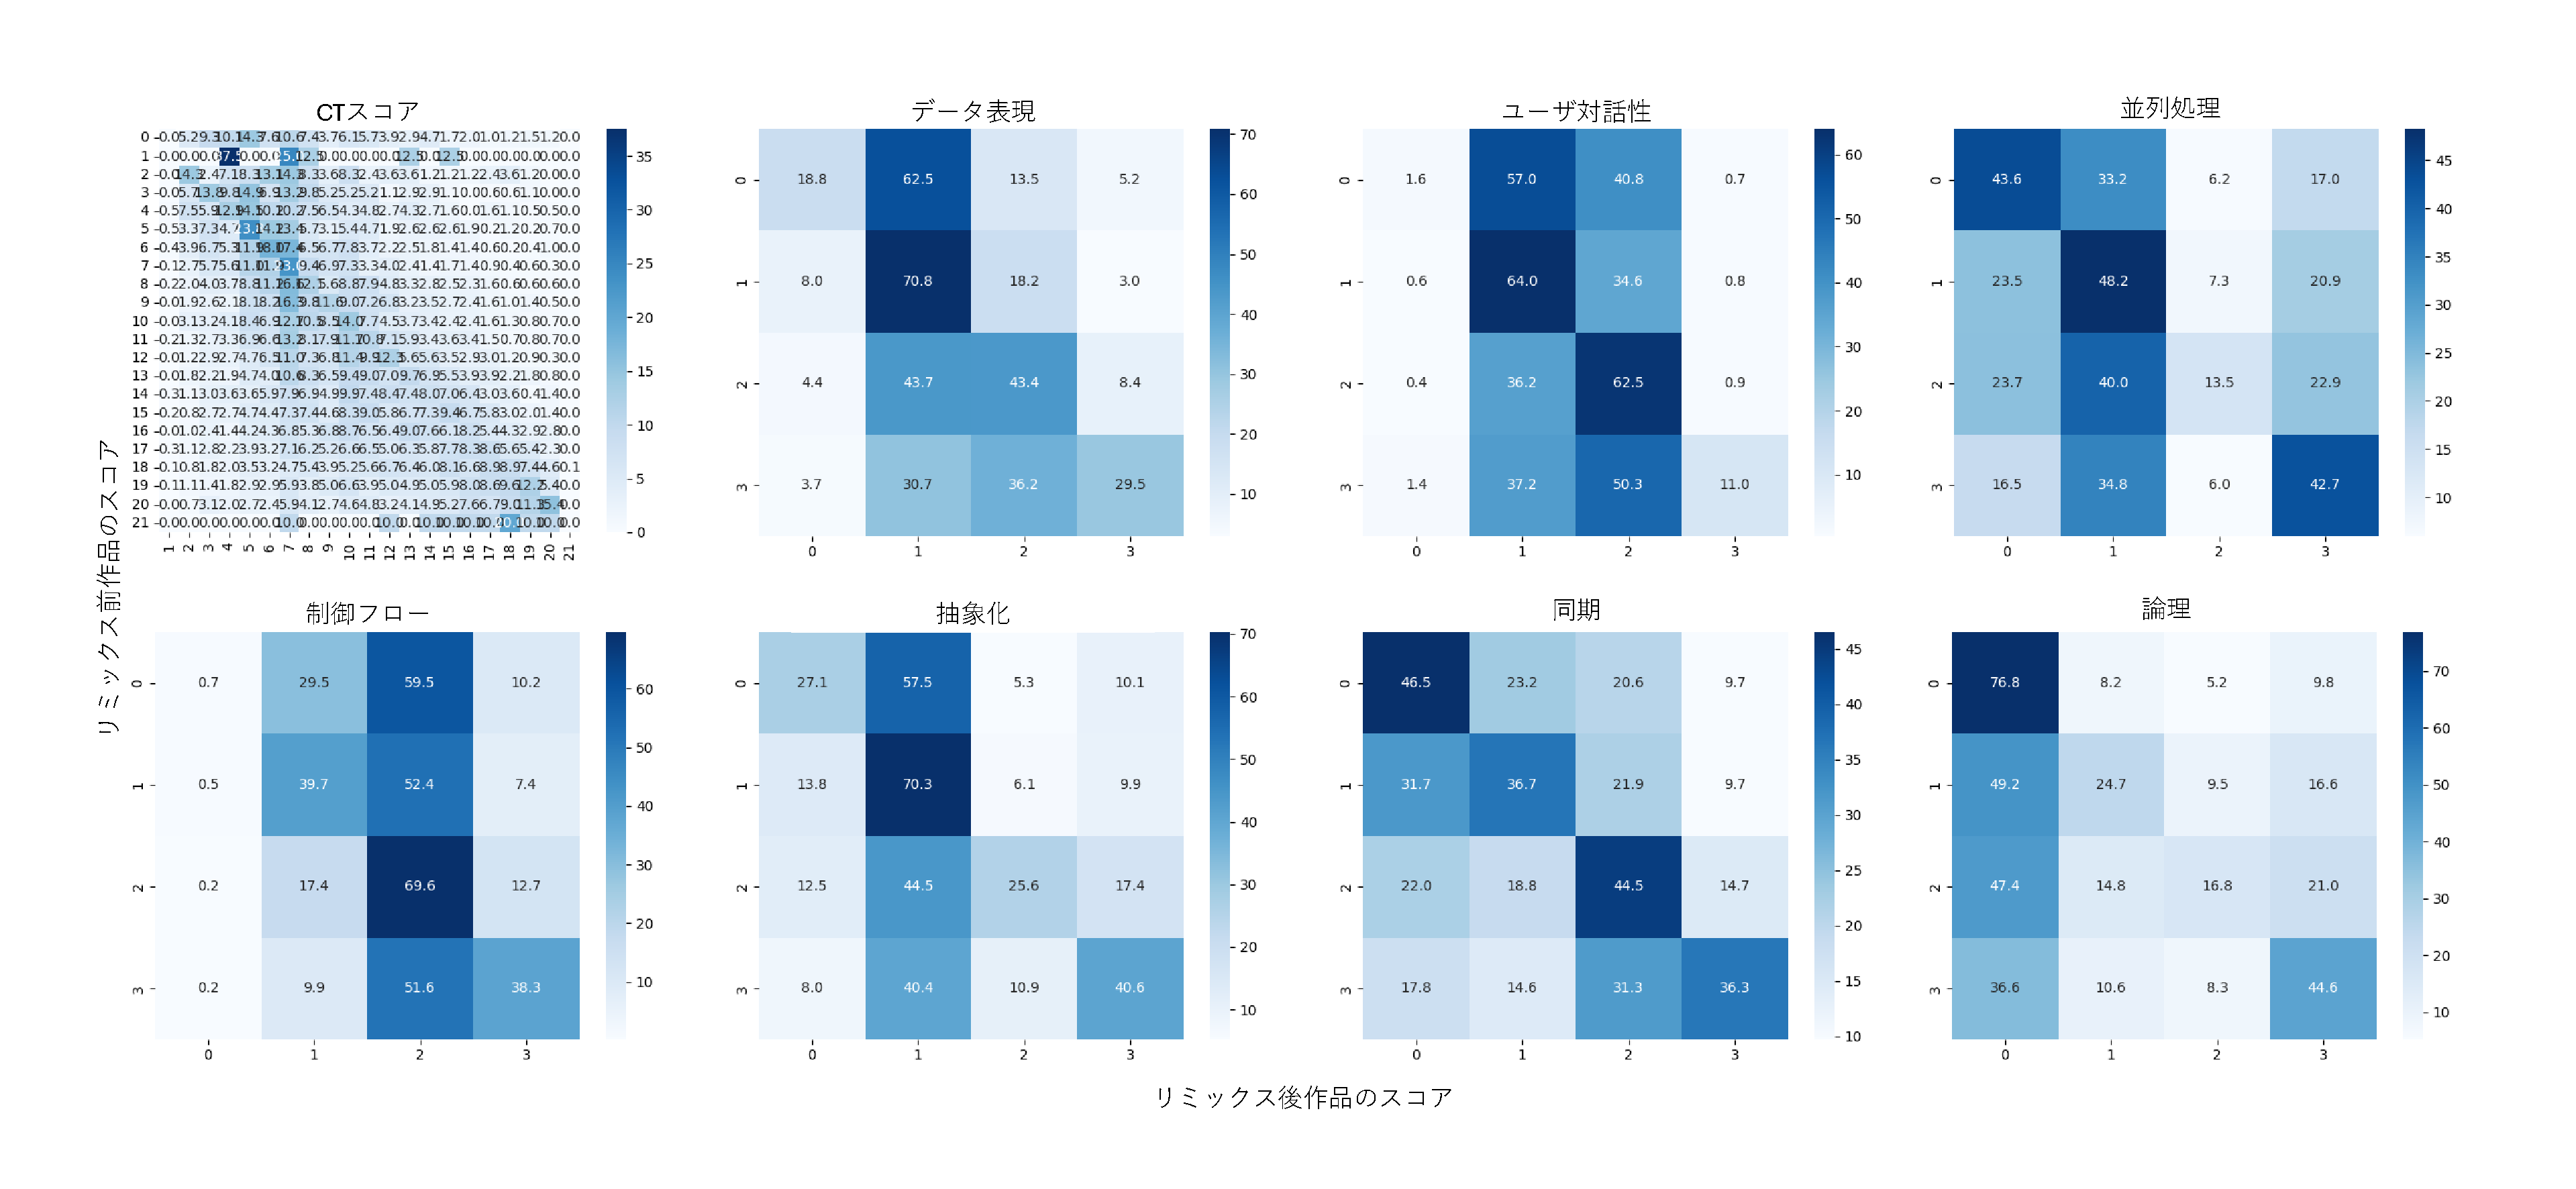
\includegraphics[width=\textwidth]{@IPSJ_SIGSE202511_Horio/heatmap.pdf}
  \caption{ヒートマップ}
  \label{heatmap}
\end{figure*}

\subsection{考察}


%%%%%%%%%%%%%%%%%%%%%%%%%%%
\section{RQ2:強化学習によるモデルは,リミックス元作品のCTスコアを適切に予測できるか}
\label{sec:rq2}
%%%%%%%%%%%%%%%%%%%%%%%%%%%

\subsection{目的}

\subsection{手法}
ユーザが作品制作した過程をマルコフ決定過程として捉え,強化学習を用いてユーザが選択するリミックス元作品のCTスコアを予測するモデルを構築するために,以下のように定義する.

\begin{itemize}
    \item 状態
        
        $s_t$:ある作品制作地点での状態(8次元)
    
        $x_t$:ある作品のCTスコア概念のベクトル(7次元)
    
        $m_t\in\{0,1\}$:リミックスであるか否か(1次元)
    
        \begin{equation}
            s_t = 
            \begin{bmatrix}
               x_t \\
               m_t 
            \end{bmatrix}
        \end{equation}

    \item 行動

        $a_t$:選択したリミックス元作品のCTスコア概念のベクトル(7次元)
    
        % $a_t$:t+1番目に制作する作品のCTスコア概念のベクトル(7次元)
      
    \item 報酬
    
        $r_t$:リミックス前後作品のCTスコアの差分のスカラー
        
        $c_t$:リミックス前作品のCTスコア
    
        $c'_t$:リミックス後作品のCTスコア
        
        \begin{equation}
            r_t = c'_t - c_t
        \end{equation}
    
        % $r_t$:前後作品のCTスコアの差分のスカラー
        
        % $c_t$:t番目の作品のCTスコア
    
        % $c'_t$:t-1番目の作品のCTスコア
        
        % \begin{equation}
        %     r_t = c'_t - c_t
        % \end{equation}

    \item 状態遷移確率
        \begin{equation}
            P(s' \mid s, a)
        \end{equation}

    \item 期待累積報酬

        $Q^{\pi}(s, a)$:期待累積報酬
    
        $\gamma$:割引率
        
        $\pi$:エージェントが従う方策

        \begin{equation}
            Q^{\pi}(s, a) = \mathbb{E}_{s' \sim P(\cdot \mid s, a)} 
            \left[ r(s, a) + \gamma \, 
            \mathbb{E}_{a' \sim \pi(\cdot \mid s')} 
            \big[ Q^{\pi}(s', a') \big] \right]
        \end{equation}

\end{itemize}

ユーザの学習過程は連続的なものであるため,強化学習はTwin Delayed DDPG(TD3)を用いる.
評価方法として,教師あり学習であるランダムフォレストと推定平均報酬の比較を行う.



\subsection{結果}

\begin{figure*}[t]
  \centering
  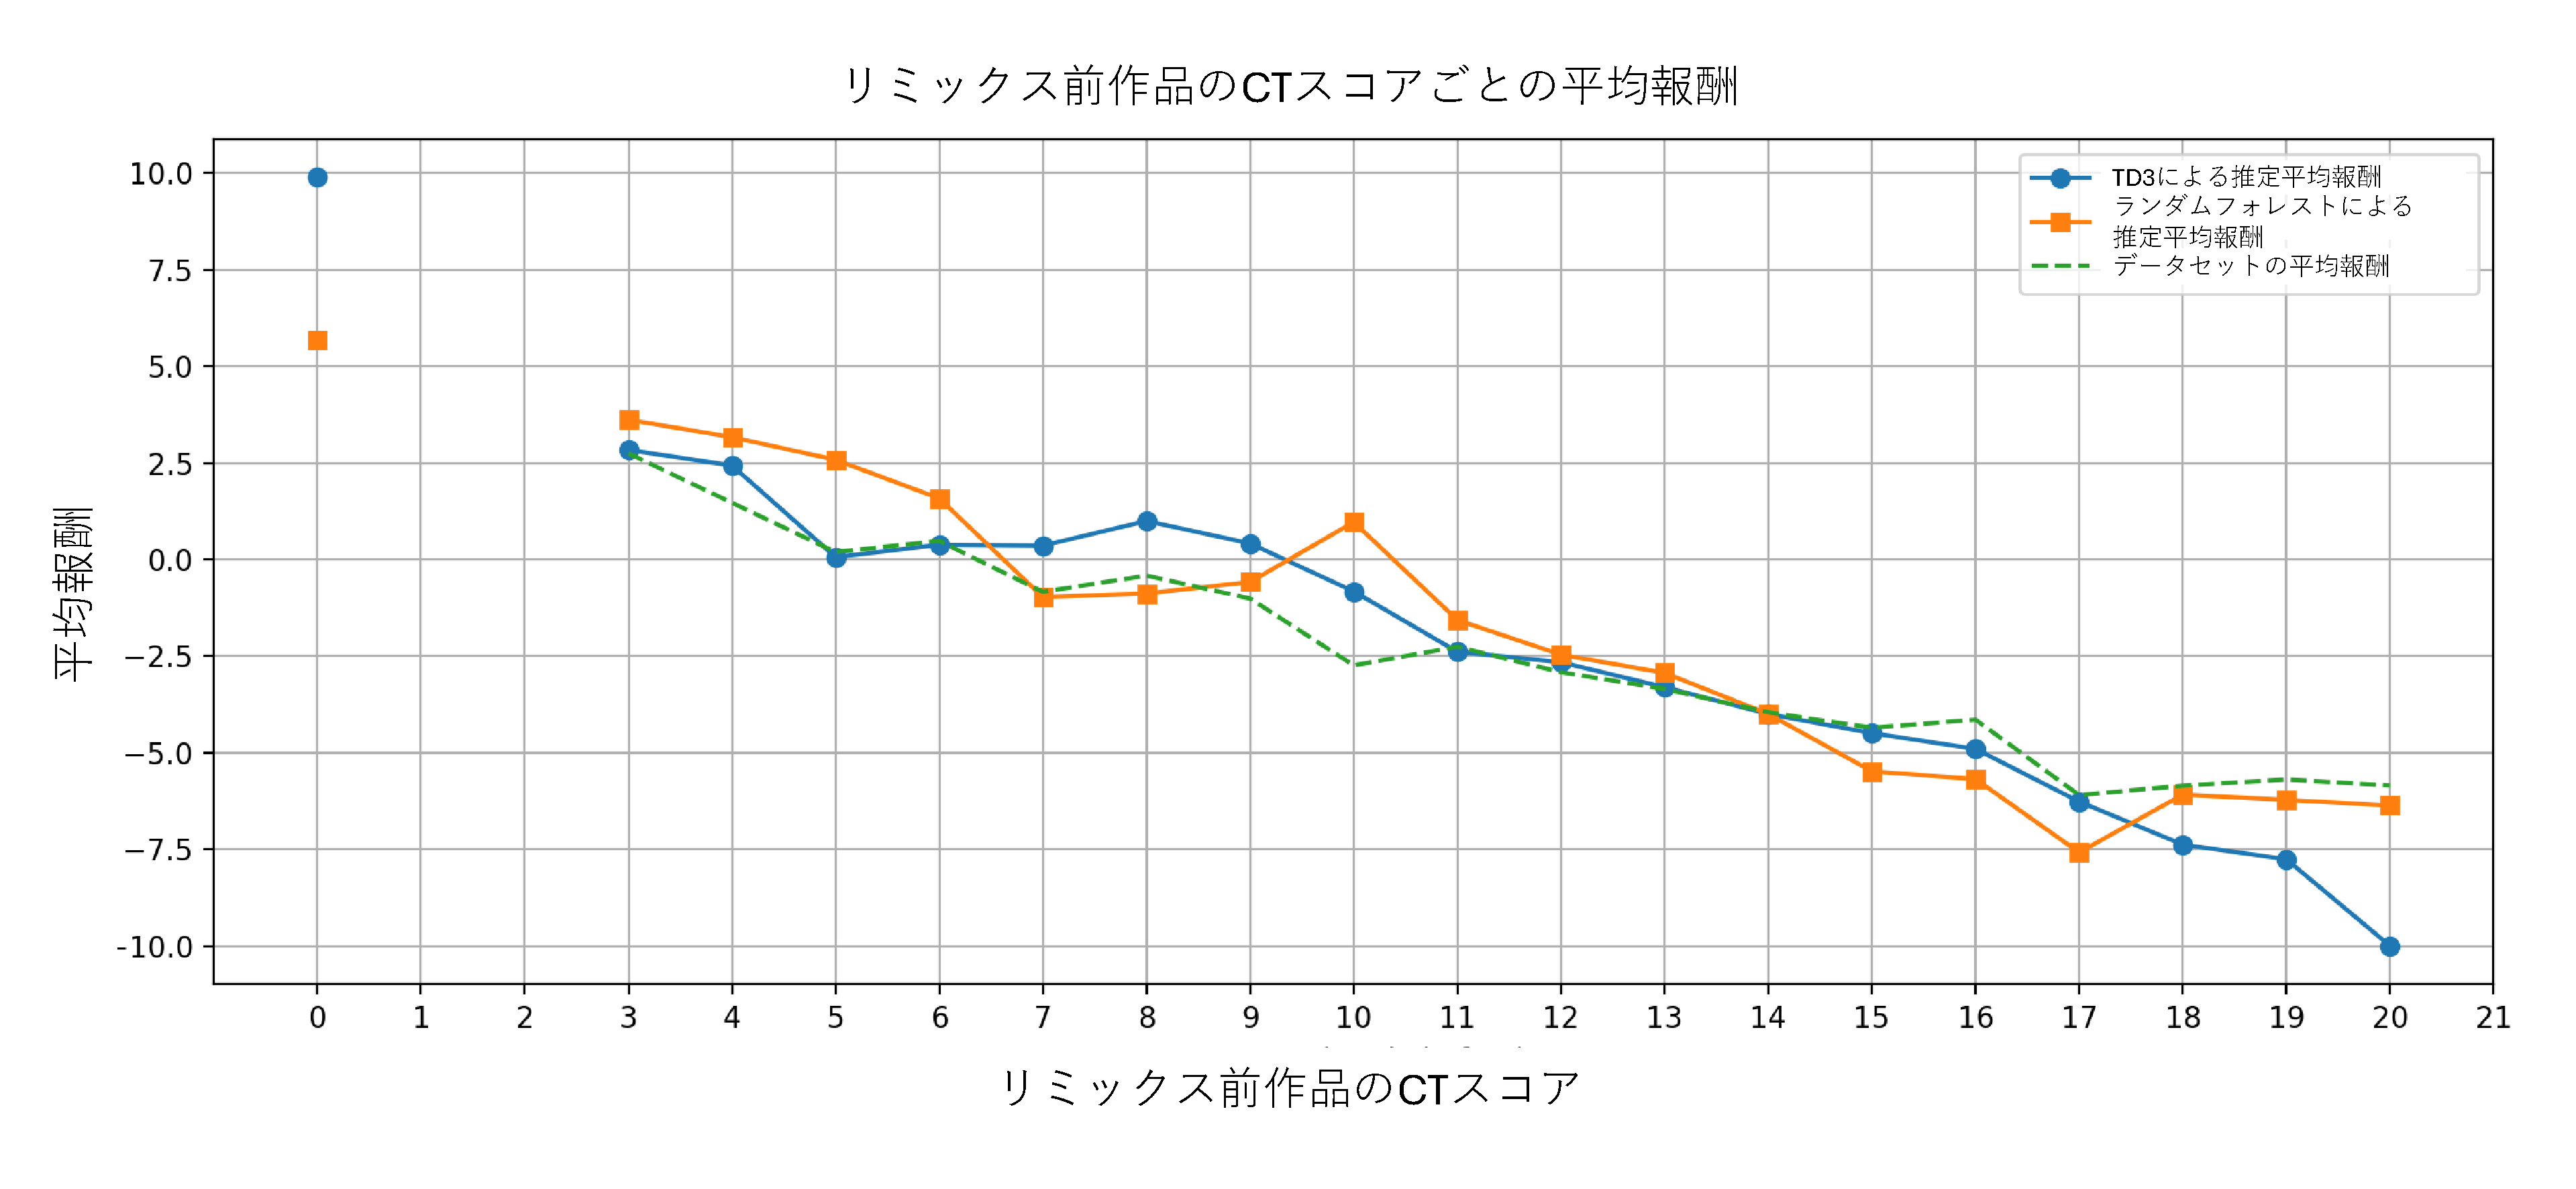
\includegraphics[width=\textwidth]{@IPSJ_SIGSE202511_Horio/estgraph.pdf}
  \caption{ESTグラフ}
  \label{estgraph}
\end{figure*}

\subsection{考察}

%%%%%%%%%%%%%%%%%%%%%%%%%%%
\section{おわりに}
\label{sec:conclusion}
%%%%%%%%%%%%%%%%%%%%%%%%%%%

\bibliographystyle{unsrt}
\bibliography{references}

\end{document}
